\chapter{Numerical simulation of time delayed gelling } \label{chap:simulation}
% -------------------------
%% QUOTE
\vspace*{\fill}
\epigraph{... in real life mistakes are likely to be irrevocable. Computer simulation, however, makes it economically practical to make mistakes on purpose. If you are astute, therefore, you can learn much more than they cost. Furthermore, if you are at all discreet, no one but you need ever know you made a mistake.}%
{\textit{Natural Automata and Useful Simulations}\\ \textsc{John H. Mcleod}}
\clearpage{\thispagestyle{empty}\cleardoublepage}
%%
%% Body of the chapter
%%%%%%%%%%%%%%%%%%%%%%
\section{Simulator development at SINTEF Industry}
The following is a description of a model, developed at SINTEF Industry, for incompressible two-phase Darcy flow (water and oil) where the water phase can contain two solutes, nanoparticles and polymers. The novel feature of the presented model is that the nanoparticles can act as time-delayed cross-linkers, postponing the formation of gel. The given model has also been discretized and implemented as a c-code. A documentation of input and output of this program is also given.

\subsection{Background}
The presented model is spatially 1-dimensional with rate-controlled injection. Thus, the model is most appropriate for simulation of core flooding experiments with specified injection rates. At present, the given version of the model does not contain capillary forces nor gravity. However, the formulation of transport properties can be generalized to more spatial dimensions, to include capillary forces and gravity, and to include the possibility of pressure-controlled boundary conditions. 

The model also contains other features (in addition to age tracking of nanoparticles) such as adsorption and possible desorption of nanoparticles and polymers, inaccessible pore space for nanoparticles and polymers, shear thinning, and absolute permeability reduction as a function of adsorbed polymer concentration. 

The water viscosity at a given location and time is a function of polymer concentration, nanoparticle concentration, the local age profile of the nanoparticles, as well as the rate. With no nanoparticles present, the formulation of the water viscosity as a function of polymer concentration corresponds to the fully mixed Todd-Longstaff formulation. When gelling is possible (i.e. when sufficiently aged nanoparticles and polymers are present), the water viscosity is interpolated between its value corresponding to no gelling and its maximal possible value (maximal gelling).  For generality, several of the input parameters defining water viscosity in the developed code are table based, allowing for flexibility in the definition of rheological properties of the water.

The numerical formulation of the presented model is standard upstream implicit Euler for the transport of water, oil, polymers, and nanoparticles, while the recalculation of the nanoparticle age distributions is done after the implicit transport equations have converged. This recalculation applies a relatively novel method \citep{Flatten2008} by treating the upstream terms explicit and the downstream terms implicit. This approach givens stability and limited dispersion. 

Since the model is spatially 1-dimensional, the Jacobian matrix in the Newton iteration has a block structure enabling a non-iterative robust and effective linear solver. Indeed, numerical simulations demonstrate robust stability due to the implicit formulation for fluid transport, and the simulator is numerically effective allowing for short timesteps in order to limit numerical dispersion inherent in the implicit formulation.

\subsection{Defining equations}
We consider an immiscible two-phase (water and oil) 1D model with injection of nanoparticles and polymer in solution with water, where capillary and gravitational forces are ignored. We will assume that polymer and sufficiently old nanoparticles forms gel, increasing the water viscosity significantly. The boundary conditions are given by specifying an (time dependent) input rate. 

\subsection{Conservation laws}
Mass conservation \index{mass conservation} for oil and water read
\begin{equation} \label{eq:massConservation} % eq 5.1
    \phi\frac{\partial S_i}{\partial t}+\frac{\partial u_i}{\partial x} = 0,\quad i = o, w
\end{equation}
where $\phi$ is the constant porosity (porosity for oil and water), $S_i=S_i(x,t), i = o,w$ are the phase saturations and $u_i, i=o,w$ are the phase volumetric fluxes. These fluxes are given by Darcy’s law \index{Darcy’s law}
\begin{equation} \label{eq:fluxes} % eq 5.2
    u_i= -k\frac{k_{ri}}{\mu_i}\frac{\partial P}{\partial x},\quad i = o, w
\end{equation}
where $P=P(x,t)$  is the pressure and $k$ is the absolute permeability. Here absolute permeability is a tabulated function of absorbed polymer concentration. Furthermore, $k_{ri}, i = o, w$ are the relative permeabilities to oil and water, which are functions of water saturation. In the present formulation, these relative permeabilities are of Corey type
\begin{subequations}
\begin{eqnarray}
 k_{rw}(S_w)=k^0_{rw}(\frac{S_w-S_{wi}}{1-S_{wi}-S_{or}})^{\alpha_w} ,\\
    k_{ro}(S_w)=k^0_{ro}(\frac{1-S_{or}-S_{w}}{1-S_{wi}-S_{or}})^{\alpha_o} ,
\end{eqnarray}
\end{subequations}
where $S_w\in [S_{wi}, 1-S_{or}]$. Here $S_{wi}$ and $S_{or}$ and are the irreducible water saturation and the residual oil saturation, $k^0_{ri}, i=o,w$  are the endpoint relative permeabilities, and , $\alpha_w$ and $\alpha_o$  the Corey exponents for water and oil. The oil viscosity $\mu_o$ is assumed constant, while the water viscosity $\mu_w$ will be a function of nanoparticle and polymer concentration, the nanoparticle age profile, as well as the flow rate. The calculation of water viscosity is presented in the next section.
Mass conservation of nanoparticles and polymers are given by 
\begin{equation} \label{eq:massConsNPpol} % eq 5.3
    \frac{\partial}{\partial t}(C_i\phi^{(i)}S_w + C_{ai}(1-\phi^{(i)})\rho_r)+ \frac{\partial}{\partial x}(C_i u_w) = 0, \quad i = n, p
\end{equation}
where $C_i=C_i(x,t), i=n,p$ are nanoparticle and polymer concentrations (molar or by weight), $C_{ai}=C_{ai}(C_i), i=n,p$ , are the adsorbed concentrations per mass of the rock for nanoparticles and polymers, $\phi^{(i)}, i=n,p$ , the porosities (accessible pore spaces) for nanoparticles and polymers, and finally, $\rho_r$ is the rock mass density. As indicated, the adsorbed concentrations are functions of their respective concentrations in the water phase, where the components can desorb or not depending on input choice. Thus, in case of no desorption, the adsorbed concentration is a hysteretic quantity.   
In addition to calculating the saturations and concentrations, we need to keep track of the local age profiles of the nanoparticles, both the age profile in the water phase and the age profile of the adsorbed nanoparticles (the adsorbed age profiles are needed if nanoparticles can desorb). This age tracking is realized by formulating a conservation scheme for nanoparticles of the same age.   

Let  $p(x,t;\tau)$ denote the age distribution of nanoparticles in solution at position  and time  . That is, 
\begin{equation*}
    p(x,t;\tau)\Delta\tau
\end{equation*}
is the fraction of nanoparticles having age in the interval $[\tau, \tau+\Delta\tau]$  at position $x$ and at time $t$. Thus $p(x,t;\tau)\geq 0$ and $\int_{0}^{\infty}{p(x,t;\tau)d\tau}=1$ . In case all nanoparticles at a location have aged more than a maximal age $T_1$, the age where maximal gel strength can be achieved, the age profile is given by the delta function $\delta(\tau-T_1)$. The age distribution of adsorbed nanoparticles at position $x$ at time $t$ is similarly given by $q(x,t;\tau)$. Thus, the total concentration of nanoparticles per bulk volume of age  $[\tau, \tau+\Delta\tau]$ at position $x$ at time $t$ is
\begin{equation}
    \left(p(x,t;\tau)C_n(x,t)\phi^{(n)}S_w(x,t)+q(x,t;\tau)C_{an}\left(C_n(x,t)\right)(1-\phi^{(n)})\rho_r\right)\Delta\tau
\end{equation}
The flux of nanoparticles of this age is
\begin{equation}
    p(x,t;\tau)C_n(x,t)u_w(x,t)\Delta\tau
\end{equation}
Thus, we can set up the conservation law for nanoparticles of age $[\tau, \tau+\Delta\tau]$  for determining the   $t$-evolution of $p(x,t;\tau)$ and $q(x,t;\tau)$. Exactly how this is realized will be described in the section describing the numerical realization of the mathematical model.

\subsection{Water viscosity}
The water viscosity is expressed as
\begin{equation}
    \mu_w=(1-\nu)\mu^p_w + \nu\mu_w^{\max}
\end{equation}
where $\mu^p_w$ is the water viscosity with only polymer present, $\mu_w^{\max}$ is the (constant) maximal possible value for water viscosity corresponding to maximal gel strength. $\nu\in[0,1]$ is an interpolator depending on nanoparticle and polymer concentrations and the age profile $p$, where  $\nu=0$ corresponds to no gelling, and $\nu=1$  signifies maximal gel strength.

The water viscosity with only polymer present is given by
\begin{equation}
    \mu_w^p=\mu_w^0 a(C_p) s(C_p, q_w),
\end{equation}
where $\mu_w^0$ is the water viscosity with no polymer present, $a (C_p)$ is the viscosity increase factor due to presence of polymer with no shear-thinning, while $s(C_p, u_w)$ is the viscosity decrease factor due to shear thinning. Note that the shear-thinning factor $s(C_p, u_w)$ is calculated explicitly in the numerical formulation. The two functions $a (C_p)$ and $s(C_p, u_w)$ are tabulated input parameters and can either be measured directly or calculated from some type of assumed functional form. The approach for defining the water viscosity as a function of polymer concentration resembles the fully mixed case for the Todd-Longstaff formulation \citep{Todd1972}.   

The interpolator (signifying degree of gelling) is given by
\begin{equation} \label{eq:ageEffect} % eq 5.8
    \nu=h(C_n,C_p) \int^{T_1}_{0}m(\tau)p(x,t;\tau)d\tau
\end{equation}
where $h(C_n,C_p)$ \index{$h$-function} is a tabulated function, and $m(\tau)$ a weight function defining how the age of the nanoparticles influences gel strength. The (normalized) function $m(\tau), \tau\in[0,T_1]$, measures the increase in water viscosity (that is interpolator value) as a function of nanoparticle aging. Typically $m(\tau)=0$ for $\tau\in[0,T_0]$,  $m^\prime(\tau)>0$ for $\tau\in\langle T_0, T_1\rangle$ , and $m(T_1)=1$ as illustrated in Figure \ref{fig:weightFunc}.

\begin{figure}[h]
    \centering
    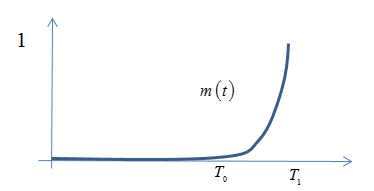
\includegraphics[width=.85\textwidth]{img/fig/weightFunc.png}
    \caption{Weight function signifying that gelling is initiated when nanoparticles have age $T_0$ and gelling reach maximal strength at age $T_1$}
    \label{fig:weightFunc}
\end{figure}

Consequently, the interpolator  $\nu$ is zero when all nanoparticles have aged less than  $T_0$. When all nanoparticles have aged more than  $T_1$, the age profile $p$ is set to  $\delta(\tau-T_1)$ , meaning that the integral in (\ref{eq:ageEffect}) satisfies $\int^{T_1}_{0}m(\tau)p(x,t;\tau)d\tau=1$ , giving the maximal value for this integral. We will refer to the integral in (\ref{eq:ageEffect})  as \textit{the age effect} (at position $x$ at time $t$ ). The function $m(\tau)$ must be measured or estimated keeping the nanoparticle and polymer concentrations constant. At this stage, we have assumed  $m(\tau)$ is independent of concentrations, but it would be straightforward to extend this function to depend on more variables. The other factor in (\ref{eq:ageEffect}), $h(C_n,C_p)$ , would reflect the gel strength as a function of the concentrations when all nanoparticles have the same age, and must be measured or estimated from more basic principles. At maximal concentrations, it is assumed that $h=1$ , while $h(C_n,C_p)=0$ when either of the concentrations are zero (i.e. no gel forms). Thus, when all nanoparticles have aged more than $T_1$, and when the nanoparticle and polymer concentrations sufficiently high (i.e. when $h(C_n,C_p)=1$ ), the interpolator is unity giving maximal value for water viscosity.

\section{Numerical realization, a summary}
It is important to formulate a numerical scheme that is as stable as possible. Consequently, the coupled conservation laws for water saturation, polymer-, and nanoparticle concentrations are solved numerically using (mainly) an implicit scheme. As the model is spatially 1D, not too many numerical grid blocks are needed, even for a fine spatial resolution. Few grid blocks also allow for using a small maximal time step without forbiddingly long simulations time. Therefore, the inherited numerical diffusion in implicit schemes can be limited by demanding short time steps, and using a first order implicit scheme (backward Euler) is sufficient for obtaining satisfactory precision. Also, the 1D formulation results in a block structured Jacobi matrix (tri-block diagonal) in the Newton iterations, allowing for a generalization of the well-known explicit solution of linear equations when the coefficient matrix is tri-diagonal. Consequently, the solver for linear equations is non-iterative, very robust, and fast. 

Not all terms are treated implicitly. The age effect $\int^{T_1}_{0}m(\tau)p(x,t;\tau)d\tau$ is updated at the end of the time step, meaning that only the factor $h(C_n,C_p)$ in (\ref{eq:ageEffect}) is treated implicitly. The age distributions $p$ and $q$ are also recalculated at the end of the time step using “mass conservation” for nanoparticles of the same age, and then adding the time step length to the age of all present nanoparticles. Incidentally, problems were encountered when solving for the “mass conservation” of the variously aged nanoparticles.  An explicit scheme for solving for the transport of various aged nanoparticles rendered unstable, while a fully implicit scheme gave rise to forbiddingly high numerical dispersion. However, by using an explicit upstream and implicit downstream seems to give excellent profiles for the age distributions. A Google search for this explicit upstream, implicit downstream approach actually revealed one single previous paper on this topic \citep{Flatten2008}. 

We first describe how the conservation equations are solved numerically, and then define how the age profiles are updated and how the age effect is calculated.

\subsection{Conversion equations}
The phase \index{mobility} mobilities are defined as
\begin{equation}
    \lambda_i = \frac{k_{ri}}{\mu_i}, \quad i=w,o
\end{equation}
First, we eliminate the pressure from the system of equations to obtain the standard Buckley-Leverett formulation. Adding the two equations given by (\ref{eq:massConservation}), and using $S_w+S_o=1$ we obtain $\frac{\partial}{\partial x}(u_w+u_o)=0$  which means that $u_T=u_w+u_o=u_T(t)$  , where $u_T$ is the total volumetric flux defined by the boundary conditions. From (\ref{eq:fluxes}) we then solve for the pressure (-derivative)
\begin{equation} \label{eq:pressureDerivative} % eq 5.9
    \frac{\partial P}{\partial x} = -\frac{u_T}{k\lambda_T}
\end{equation}
where  $\lambda_T=\lambda_w+\lambda_o$ is the total mobility. In particular, (\ref{eq:pressureDerivative}) is used for calculating the pressure after a converged time step. Note that the absolute permeability only enters in the model through (\ref{eq:pressureDerivative}) (not in the system of equations we solve) when the pressures are calculated for reporting purposes. Indeed, when using rate controlled boundary conditions and incompressible flow, the pressure is not “an issue” as it is eliminated by (\ref{eq:pressureDerivative}) from the set of equations. Also, note that total volumetric flux $u_T(t)$ in (\ref{eq:pressureDerivative}) is given from the input data, not calculated. From (\ref{eq:massConservation}) with  $i=w$ we then obtain
\begin{equation} \label{eq:fractionalFlow} % eq 5.10 
    \phi\frac{\partial S_w}{\partial t}+u_T(t)\frac{\partial f_w}{\partial x} = 0
\end{equation}
where $f_w=\frac{\lambda_w}{\lambda_T}$ is the fractional flow of water. The mass conservation equations for nanoparticles and polymers given by (\ref{eq:massConsNPpol}) are then expressed as
\begin{equation} \label{eq:longMassConservation} % eq 5.11
    \frac{\partial}{\partial t}\left( C_k\phi^{(k)}S_w + C_{ak}(C_k)(1-\phi^{(k)}) \rho_r \right) + u_T(t) \frac{\partial}{\partial x}(C_k f_w)=0, \quad k=n,p
\end{equation}
The three equations given by (\ref{eq:fractionalFlow}) and (\ref{eq:longMassConservation}) are coupled and non-linear, and are solved for $S_w$, $C_n$ and $C_p$  using Euler’s backward method, with the explicit exceptions referred to earlier.

Given  $\Delta x$ and $\Delta t$ ($\Delta t$  varies in general for different time steps, while $\Delta x$ is assumed constant) at time $t=t^n$ , we let $S_w(i\Delta x, t_n+\Delta t) \approx S_i^{n+1}$ , and similarly for the other space and/or time dependent variables. Equation (\ref{eq:fractionalFlow}) becomes
\begin{multline}% eq 5.12
    E_i \left(S^{n+1}_{i-1}, C^{n+1}_{\textit{NP}, i-1}, C^{n+1}_{pol, i-1}, S^{n+1}_{i}, C^{n+1}_{\textit{NP}, i}, C^{n+1}_{pol, i}\right)  = \\ \phi\frac{S^{n+1}_{i}-S^{n}_{i}}{\Delta t} +u_T^{n+1}\frac{f_i^{n+1}\left(S^{n+1}_{i}, C^{n+1}_{\textit{NP}, i}, C^{n+1}_{pol, i}  \right) - f_{i-1}^{n+1}\left(S^{n+1}_{i-1}, C^{n+1}_{\textit{NP}, i-1}, C^{n+1}_{pol, i-1}  \right)}{\Delta x}  = 0 \\
    \quad
\end{multline} 
where we have dropped the $w$  index for water saturation and fractional flow. In simulations, the time step is such that the total rate  $u_T$ is constant in the corresponding time interval. We have assumed the direction of flow is with increasing spatial index value $i$ , and the water fractional flow is as indicated calculated using upstream weighted mobilities. As discussed, the water viscosity, and therefore the water fractional flow $f$, is not entirely implicitly calculated, as the age-profiles $p$ and the shear-thinning effect are treated explicitly.

The flux term in equation (\ref{eq:longMassConservation}) is also given by upstream weighting (assuming flow in direction of increasing index $i$ )
\begin{equation}
\begin{split}
    F_{k,i}\left(S^{n+1}_{i-1}, C^{n+1}_{\textit{NP}, i-1}, C^{n+1}_{pol, i-1}, S^{n+1}_{i}, C^{n+1}_{\textit{NP}, i}, C^{n+1}_{pol, i}\right) = u_T^{n+1} \frac{C^{n+1}_{k,i} f^{n+1}_{i} - C^{n+1}_{k,i-1} f^{n+1}_{i-1}}{\Delta x},\\  k=n,p \\ \quad
\end{split}
\end{equation}
The time derivative of the capacity term is approximated by
\begin{multline}
    G_{k,i}\left(S^{n+1}_{i}, C^{n+1}_{k,i}\right) = \\ 
    \phi^{(k)} \frac{C^{n+1}_{k,i} S^{n+1}_{i} - C^{n}_{k,i} S^{n}_{i}}{\Delta t} + \left(1-\phi^{(k)}\right) \rho_r 
    \frac{C_{ak} \left(C^{n+1}_{k,i}\right) - C_{ak} \left(C^{n}_{k,i}\right)}{\Delta t} U \left(C^{n+1}_{k,i} - C^{n}_{k,i}, w_k \right)
    ,\\ k=n,p \\ \quad
\end{multline}
where
\begin{equation*}
\begin{split}
    U(x,w) &= 1     \quad \text{if } w=0 \text{ \& } x\geq0 \text{, or if } w=1 \\
    U(x,w) &= 0     \quad \text{if } w=0 \text{ \& } x<0 
\end{split}
\end{equation*}
Here  $w_k=1$ if desorption can occur for component $k, (k=n,p)$, and $w_k=0$  if desorption does not occur.

As the model presently allows only water to be injected, we have  $q_T^{n+1}=\frac{Q_w^{n+1}}{A}$, where $Q_w^{n+1}$ is the given volumetric injection rate for water in the time interval $\left[t^n,t^{n+1}\right]$ , and where $A$ is the cross sectional area of the porous medium. Furthermore $f^{n+1}_0=1$,  $C^{n+1}_{k,0}=C^{n+1}_{k,inj}$, $k=n,p$, where $C^{n+1}_{k,inj}$ is the given injection concentration of component $k$ in the time interval $\left[t^n,t^{n+1}\right]$, and is constant during a time step. Let $n_x$  denote the number of grid blocks. For $i=1,2,...,n_x$, we then we have the $3n_x$  algebraic equations
\begin{equation}
    E_i \left(S^{n+1}_{i-1}, C^{n+1}_{\textit{NP}, i-1}, C^{n+1}_{pol, i-1}, S^{n+1}_{i}, C^{n+1}_{\textit{NP}, i}, C^{n+1}_{pol, i}\right)  = 0, % eq 5.15
\end{equation}
\begin{equation}
    G_{\textit{NP}, i} \left(S^{n+1}_{i}, C^{n+1}_{\textit{NP}, i}\right)+ F_{\textit{NP}, i} \left(S^{n+1}_{i-1}, C^{n+1}_{\textit{NP}, i-1}, C^{n+1}_{pol, i-1}, S^{n+1}_{i}, C^{n+1}_{\textit{NP}, i}, C^{n+1}_{pol, i}\right) =0, % eq 5.16
\end{equation}
\begin{equation}
    G_{\textit{pol}, i} \left(S^{n+1}_{i}, C^{n+1}_{\textit{pol}, i}\right)+ F_{\textit{pol}, i} \left(S^{n+1}_{i-1}, C^{n+1}_{\textit{NP}, i-1}, C^{n+1}_{pol, i-1}, S^{n+1}_{i}, C^{n+1}_{\textit{NP}, i}, C^{n+1}_{pol, i}\right) =0, % eq 5.17
\end{equation}
for the $3n_x$ unknowns $S^{n+1}_{i}, C^{n+1}_{\textit{NP}, i}, C^{n+1}_{pol, i}, i=1,2,...,n_x$.

Solving this set of non-linear equations requires use of Newton’s method for systems of equations, which again requires a new Jacobi matrix at each Newton iteration. The $3n_x \times 3n_x$   Jacobi matrix is sparse and block diagonal where the block matrices are generally $6\times6$  matrices. Due to this structure, Gauss-elimination does not destroy the sparse structure, and also the number of arithmetic operations in the Gauss-elimination only grow linearly with $n_x$. 

We will not write down the explicit formula for the Jacobi matrix as used in the computer code, but report that the Newton iteration shows excellent second order convergence using  $S^{n}_{i}, C^{n}_{\textit{NP}, i}, C^{n}_{pol, i}, i=1,2,...,n_x$   as initial guess in the iteration, which actually validates the expressions obtained and used for the various partial derivatives needed for forming the Jacobi matrix.

One can also analyze the explicit expression for the matrix to conclude that the Jacobi matrix is always not near singular, and no attempt have been made at this stage for calculating the condition number for the matrix.

It is important that  $C^{n+1}_{\textit{NP}, i}$ and $C^{n+1}_{pol, i}$ are scaled in the system of equations. This gives contributions from saturations and concentrations equal footing in the calculation of the residual in each Newton iteration.

\subsection{Updating age profiles}
\index{age function} At each position, and at each time step, the nanoparticles in solution and the adsorbed nanoparticles each have their own age profile $p$ and $q$. These age profiles are probability distributions on the interval $[0,T_1]$, \textit{i.e.}, $p\geq0$  and $\int^{T_1}_0 p(x,t;\tau)d\tau=1$  , and likewise for  $q$. No gelling (cross-linking) can occur before nanoparticles reach the minimum gelling age  $T_0$. Maximally strong gel may form at a given position and time when all the nanoparticles in solution have reached age $T_1$ (if also $h(C_n,C_p)=1$) the water reaches its maximal viscosity, see (\ref{eq:ageEffect})).

The numerical representations of $p(x,t;\tau)$ and $q(x,t;\tau)$ are given as follows: At time $t=t^n$ we let
\begin{equation}
    p(i\Delta x,t^n;\tau^r)=p^{n,r}_i, \quad i=1,2,...,n_x, \quad r=1,2,...,m^n,
\end{equation}
where $m^n$ is the number of ages at time $t^n$ , and similarly for $q$. The age profile resolution $\tau^1,\tau^2,...,\tau^{m^n}$ is dynamical, but the  $\tau$-resolution is the same for every position at a given time, both for $p$ and $q$.

At early times in the simulation, the list of ages, $\tau^1=t^n-t^{n-1},\tau^2=t^n-t^{n-2},...,\tau^{n-1}=t^n-t^1, \tau^{n}=t^n$, is defined by the length of the time steps. When the (user defined) maximum number of ages is obtained, the list of ages is recalculated. The maximal number of ages with $\tau^k<T_0$  is a given input value, and the same applies for the maximal numbers of ages for  $T_0\leq\tau^k\leq T_1$. When the maximum number of ages is reached, either ages younger than  $T_0$, or for ages in the interval $[T_0,T_1]$, the ages are redistributed evenly, and the age fractions $p$ and $q$ corresponding to the new list of ages recalculated to match the previous representation of $p$ and $q$. The recalculation of $p$ and $q$ uses linear interpolation for obtaining new values of  $p^{n,k}_i$ and $q^{n,k}_i$, and a renormalization to ensure $\sum^{m_n}_{k=1} p_i^{n,k}\Delta\tau^k=1$  and  $\sum^{m_n}_{k=1} q_i^{n,k}\Delta\tau^k=1$. When all ages of the nanoparticles in solution are older than $T_1$, the age effect entering in Equation (\ref{eq:ageEffect}), $\int^{T_1}_{0} m(\tau)p(x,t;\tau)d\tau$ is simply set to unity.

Now, assume we have obtained $S^{n+1}_{i}, C^{n+1}_{\textit{NP}, i}, C^{n+1}_{pol, i}, i=1,2,...,n_x$ at time $t=t^{n+1}$ from solving the conservation equations. In addition, we know the age distributions $p^{n,k}_i$ and $q^{n,k}_i$ at time $t=t^{n}$.

The flux of nanoparticles having age in the interval $\left[\tau^k, \tau^{k+1}\right]$ is
\begin{equation}
    p(x,t;\tau)C_n(x,t)u_w(x,t)\Delta\tau = p(x,t;\tau)C_n(x,t)u_T(t)f_w(x,t)\Delta\tau
\end{equation}
To compute the  $x$-derivative we will adopt an explicit upstream, implicit downstream method. That is, we will let
\begin{multline}
    \frac{\partial}{\partial x} \left(p(x,t;\tau)C_n(x,t)u_T(t)f_w(x,t)\Delta\tau\right) \approx \\ \frac{u_T^{n+1}}{\Delta x} \left(p_i^{n+1,k}C_{n,i}^{n+1}f_i^{n+1}- p_{i-1}^{n,k}C_{n,i-1}^{n}f_{i-1}^{n}\right)\Delta\tau
\end{multline}
Thus,
\begin{equation} \label{eq:massNP} % eq. 5.19
    u_T^{n+1} \left(p_i^{n+1,k}C_{n,i}^{n+1}f_i^{n+1}- p_{i-1}^{n,k}C_{n,i-1}^{n}f_{i-1}^{n}\right)\Delta\tau A\Delta t
\end{equation}
approximates the mass (or molar) of nanoparticles in solution of with ages in the interval $\left[\tau^k, \tau^k+\Delta\tau\right]$  flowing out of grid block $\left[x_{i-1},x_i\right],i=1,2,...,n_x$ during the time step  $\left[t^n, t^n+\Delta t\right]$. Here $A$ is the cross-sectional area of the model. As previously discussed, any other way of realizing the  $x$-derivative in (\ref{eq:massNP}) leads to non-physical results, either highly unstable (using explicit both up- and downstream) or forbiddingly dispersive (using a full implicit formulation). 

Assume first that the mass of nanoparticles flowing out of the grid block is negative. Then the nanoparticle concentration increases locally, and consequently no adsorbed nanoparticles will desorb at this position. Therefore, the age profile of the adsorbed nanoparticles $q_i^{n,k}$ at time $t^n$ will not affect the new age profile  $p_i^{n+1,k},k=1,2,...,m_{n+1}$ of the nanoparticles in solution at time  $t^{n+1}$. The mass of nanoparticles with ages in the interval $\left[\tau^k, \tau^k+\Delta\tau\right]$ is
\begin{equation*}
    \left(p(x,t;\tau)C_n(x,t)\phi^{(n)}S_w(x,t) + q(x,t;\tau)C_{an}(C_n(x,t))(1-\phi^{(n)})\rho_r\right) \Delta\tau A\Delta x
\end{equation*}
Thus, numerically the change of mass for these particles during the time step $\left[t^n, t^n+\Delta t\right]$ is
\begin{multline} \label{eq:massChangeNP} % eq 5.20
    \bigg[\phi^{(n)}\left(p_i^{n+1,k}C_{n,i}^{n+1}S_i^{n+1}- p_{i}^{n,k}C_{n,i}^{n}S_{i}^{n}\right) +\\ \rho_r(1-\phi^{(n)}) \left(q_i^{n+1,k}C_{an}(C_{n,i}^{n+1})- q_{i}^{n,k}C_{an}(C_{n,i}^{n})\right)\bigg]
    \Delta\tau A\Delta x
\end{multline}
We can eliminate $q_{i}^{n+1,k}$ by noting that the increased mass of adsorbed nanoparticles at this time step is
\begin{equation*}
    \left(C_{an}(C_{n,i}^{n+1})- C_{an}(C_{n,i}^{n})\right)
    \rho_r\left(1-\phi^{(n)}\right) A\Delta x
\end{equation*}
Thus, the increased mass of absorbed nanoparticles (which all come from the nanoparticles in solution) with ages in the interval $\left[\tau^k, \tau^k+\Delta\tau\right]$ is
\begin{equation*}
    p_i^{n+1,k}\left(C_{an}(C_{n,i}^{n+1})- C_{an}(C_{n,i}^{n})\right)
    \rho_r\left(1-\phi^{(n)}\right) A\Delta x.
\end{equation*}
Writing down mass conservation for absorbed nanoparticles of this age we find
\begin{multline} \label{eq:elimiateQ} % eq 5.21
    p_i^{n+1,k}\left(C_{an}(C_{n,i}^{n+1})- C_{an}(C_{n,i}^{n})\right)
    \rho_r\left(1-\phi^{(n)}\right) A\Delta x + \\
    C_{an}(C_{n,i}^{n})\rho_r\left(1-\phi^{(n)}\right)q_i^{n,k} = \\
    C_{an}(C_{n,i}^{n+1})\rho_r\left(1-\phi^{(n)}\right)q_i^{n+1,k}A\Delta x 
\end{multline}
Using (\ref{eq:elimiateQ}) we can then eliminate $q_i^{n+1,k}$ in (\ref{eq:massChangeNP}). 

Thus, formulating the mass conservation for nanoparticles of age $\left[\tau^k, \tau^k+\Delta\tau\right]$ using (\ref{eq:massNP}) and (\ref{eq:massChangeNP}) (having eliminated  $q_i^{n+1,k}$) we simply obtain an explicit formula $p_i^{n+1,k}$. Then from (\ref{eq:elimiateQ}) we find the values for $q_i^{n+1,k}$.

Assume now that the mass of nanoparticles decreases at a given position during a time step, \textit{i.e.}, that (\ref{eq:massNP}) is positive. Then if the option for no desorption of nanoparticles is set, the age profile for the adsorbed nanoparticles stays the same (except that all the adsorbed nanoparticles age the amount of the time step), and $C_{an}(C_{n,i}^{n+1})- C_{an}(C_{n,i}^{n})=0$. Thus (\ref{eq:elimiateQ}) is satisfied, and $q_i^{n+1,k}=q_i^{n,k}$, and the mass conservation for $p_i^{n+1,k}$ can be solved directly.

If desorption of nanoparticles can occur, then (\ref{eq:elimiateQ}) still applies, and $p_i^{n+1,k}$ and  $q_i^{n+1,k}$ can be found as previously described for the case when (\ref{eq:massNP}) is negative. 

We also observe that the procedure for updating the age profiles is done independently for each $k$.

In (\ref{eq:massNP}) for $i=1$, the age profile for the injected nanoparticles, $p_0^{n,k}$, has $p_0^{n,1}=1$ and $p_0^{n,k}=0$ for $k\geq2$. That is, all injected nanoparticles have minimum age. Note that it is simple to modify the model to allow for a general user defined age profile of the injected nanoparticles.

When $p_i^{n+1,k}$ and $q_i^{n+1,k}$ have been determined, the ages the distributions represent are of course increased by one time step, and the  $k$-index shifted one up. In fact, when the user defined maximal number of ages is reached, the computer code will always recalculate the representations of the age profiles as previously described, since adding a new age will exceed the maximal number of ages.

Finally, the age profile $p_i^{n+1,k},k=1,2,...,m_{n+1}$,  is used for estimating the integral
\begin{equation}
    \int_{T_0}^{T_1} m(\tau)p(x,t;\tau)d\tau
\end{equation}
\textit{the age effect}.

Since $m$ and $p$ generally are represented with values at different nodes, we linearly interpolate $p$ to match the nodes where $m$ is given, and calculate the integral using the trapezoidal method. This value for the age effect is then used in the upcoming new time step, where the other parameters defining water viscosity are treated implicitly in this new next time step (except the shear thinning effect).

\subsection{Table based input}
A number of the functions needed for the model are table based allowing for input generality. These functions constitute part of the input for the model, and must be measured in the laboratory or estimated from physical principles. All tabulated functions are either functions of one or two variables. Numerical noise may result in function calls outside the given domain, which could lead to ambiguities and possible failure of simulation. For functions of a single variable (defined on an interval) the code will both interpolate and extrapolate linearly. However, the program issues a warning when it has to extrapolate a function outside its given domain, reporting which function and which out of domain argument value it extrapolates to.

Two-variable functions are defined on a rectangle $\big[a,b\big]\times\big[c,d\big]$. Two-variable functions are evaluated by successive linear interpolation. Concerning extrapolation outside the domain of definition, for an argument $(x,y)$ which both has $x\notin\big[a,b\big]$ and $y\notin\big[c,d\big]$, the error will be fatal, and the program stops. In case of membership in only one of the intervals, the code will extrapolate linearly and report a warning.

Also, the various derivatives of table defined functions are needed for the Jacobi matrix. The derivatives are piecewise constant, and are calculated consistently with the linear interpolation of function values. Regarding extrapolation of derivatives, the values of derivatives are simply extended constantly outside their domains, both the ordinary and the partial derivatives.

As mentioned so far, the Newton iterations behave excellent showing second order convergence. This indicates that the implemented formulation and evaluation of function values and derivatives of table based functions is sound and robust.   


\section{Initial testing of 1D simulator}

Input to the simulator is text based and input functions are tabulated. For example, the change of water viscosity as function of polymer concentration is given as a table with polymer concentration in the first column and relative change in viscosity for the water in the second column. An example input file for the simulator with comments describing each input parameter is listed in Appendix \ref{chap:simInput}. 

The simulation grid is defined by number of grid blocks ($n_x$), the length of the model and the cross-sectional area of the model. Porosity and permeability is given by constants for the whole model. When nanoparticles or polymer is present in the water phase, inaccessible pore volume (IPV) can be defined to reduce the porosity for these particles in solution. Initial water saturation can be given explicitly for each grid block ($n_x$-values) or as a constant for the model, oil saturation is calculated from water saturation. Simulations reported here has no oil in the models.

Saturation functions (relative permeability functions) for oil and water are of Corey-type and are defined in the input file by parameters for residual saturations, end point values and Corey exponents (three parameters for each phase). Mobility change for the water phase is modelled through change in viscosity as function of polymer concentration and when gelling occurs. Relative change in water viscosity as a function of polymer concentration is given as a table input. Reduction in viscosity for water with polymer due to shear thinning is given as a two-variable tabulated function of polymer concentration and relative rate (relative to a reference rate given as input).   

The \index{$h$-function} $h$-function and the \index{age function} age function responsible for the gelling effect as described in the previous section are given as a two-variable tabulated function of polymer and nanoparticle concentration and a tabulated function of time, respectively. 

Oil viscosity is set constant. However, the absolute permeability can be reduced by adsorbed polymer, affecting the effective oil and water mobility. Adsorption and desorption isotherms for polymer and nanoparticles are given as tabulated functions of concentration. Desorption can be turned off in the input file.

Boundary condition at the outlet of the model is specified as a constant pressure boundary. Boundary conditions at the inlet are in general time dependent (rate controlled) and are specified within a given time interval by solution (water) injection rate, concentration of nanoparticles injected in solution and concentration of polymer injected in solution. Any number of consecutive boundary control statements (time intervals) can be given. 

In addition, simulator specific input parameters such as upper and lower constraints for time steps, maximum number of linear and nonlinear iterations, time step controls and maximum water viscosity change must be set. All input parameters except simulator specific parameters such as number of grid blocks, time step constraints, convergence criteria and print out frequency/format are taken from experiments. 

To investigate numerical dispersion and effect of adsorption, the simulator was tested with varying parameters for time step constraints, number of grid blocks and adsorption coefficients, this was done for the case of nanoparticle injection in Bentheimer. An overview of sensitivity simulations are listed in Table \ref{tab:simSensitivity}.
Schedule input for these simulations are: Inject a slug of 2.28 pore volumes (PV) 1000 ppm nanoparticle (NP) solution, followed by 1.8 PV synthetic sea water (SSW), again followed by 3.47 PV 100 ppm nanoparticle solution and finally 1.71 PV SSW. 

\begin{table}[h!]
\small
\centering
\caption{Sensitivity simulations investigating numerical dispersion (time step and number of grid blocks) and the effect of adsorption and desorption}
\label{tab:simSensitivity}
\begin{tabular}{l l l l l } 
\toprule
\footnotesize\textbf{Simulations} & \footnotesize\textbf{Number of} & \footnotesize\textbf{Max time step} & \footnotesize\textbf{Adsorption } & \footnotesize\textbf{Desorption}  \\ 
\scriptsize(number of sim.) & \footnotesize\textbf{grid blocks } & \footnotesize\textbf{length }[hrs]& & [on/off] \\
\midrule 
\scriptsize Sensitivity 1 (6)  & \cellcolor{gray!15}10-2048   & 0.01       & $9.37\cdot10^{-6}$ & off \\
\scriptsize Sensitivity 2 (4)  & 120       & \cellcolor{gray!15}0.001-0.05 & $9.37\cdot10^{-6}$ & off \\ 
\scriptsize Sensitivity 3 (4)  & 120       & 0.01       & \cellcolor{gray!15}\tiny $9.37\cdot10^{-6} -3.0\cdot10^{-
5}$ & off \\ 
\scriptsize Sensitivity 4 (2)  & 120       & 0.01       & $9.37\cdot10^{-6}$ & \cellcolor{gray!15}on/off \\
\bottomrule
\end{tabular}
\end{table}

To investigate the result of the sensitivity simulations, nanoparticle concentration in the last grid block (outlet of the model) is reported. This is one of the main quantities that is measured from the experiments in addition to differential pressure over the core. However, all properties (pressure, saturations, concentrations, viscosity, age profiles, etc.) can be reported for each grid block at each reporting time step. 
The result of changing number of grid blocks and maximum time step length are shown in Figure \ref{cht:simNP}. For small number of grid blocks, the numerical dispersion is apparent as it smooths the nanoparticle concentration response (Figure \ref{cht:simNPa}) resulting in a too early breakthrough of the nanoparticles. The same can be seen if the maximum time step length is too high (Figure \ref{cht:simNPb}). For number of grid blocks above 120 and maximum time step length smaller than 0.1 the numerical effects seem to be acceptable. The effect of changing the adsorption isotherm and including desorption is shown in Figure \ref{cht:simNPconc}. Increasing the adsorption shifts the breakthrough of nanoparticles in the first slug. Without desorption, the response in the second slug is not affected since maximum amount of nanoparticles is adsorbed on the surface of the rock in the first slug (Figure \ref{cht:simNPconcA}). If desorption is switched on in the simulation the second slug will also be affected as nanoparticles have been desorbed during flooding with SSW (Figure \ref{cht:simNPconcB}). 

\begin{figure}[h] % figure 6.2
    \begin{subfigure}{\textwidth}
    \centering
    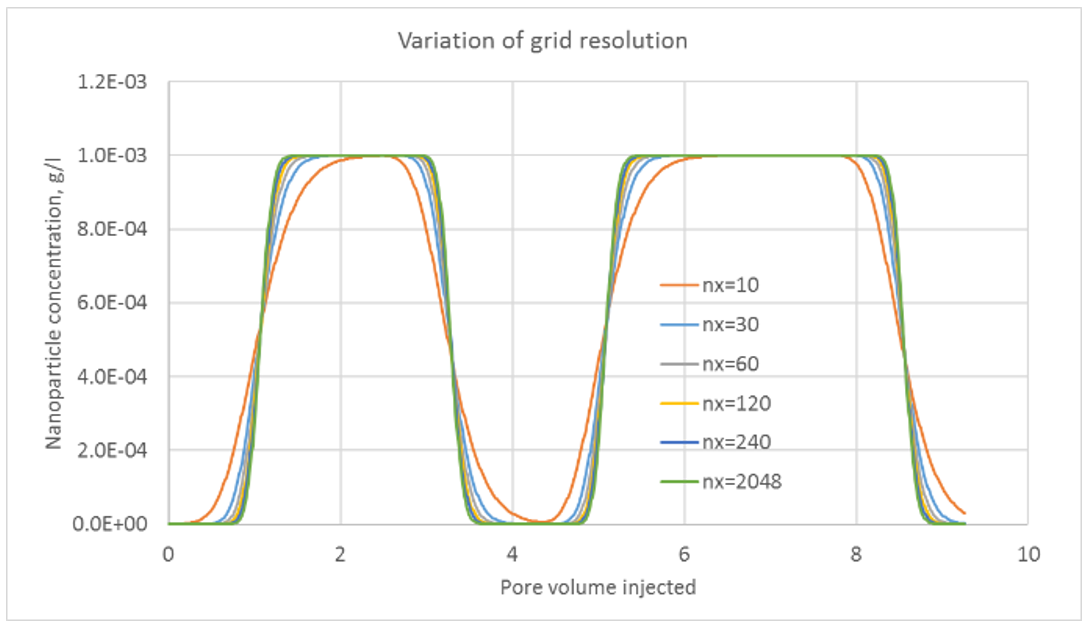
\includegraphics[width=\textwidth]{img/cht/simNPa.png}
    \caption{}
    \label{cht:simNPa}
    \end{subfigure}
    \\
    \begin{subfigure}{\textwidth}
    \centering
    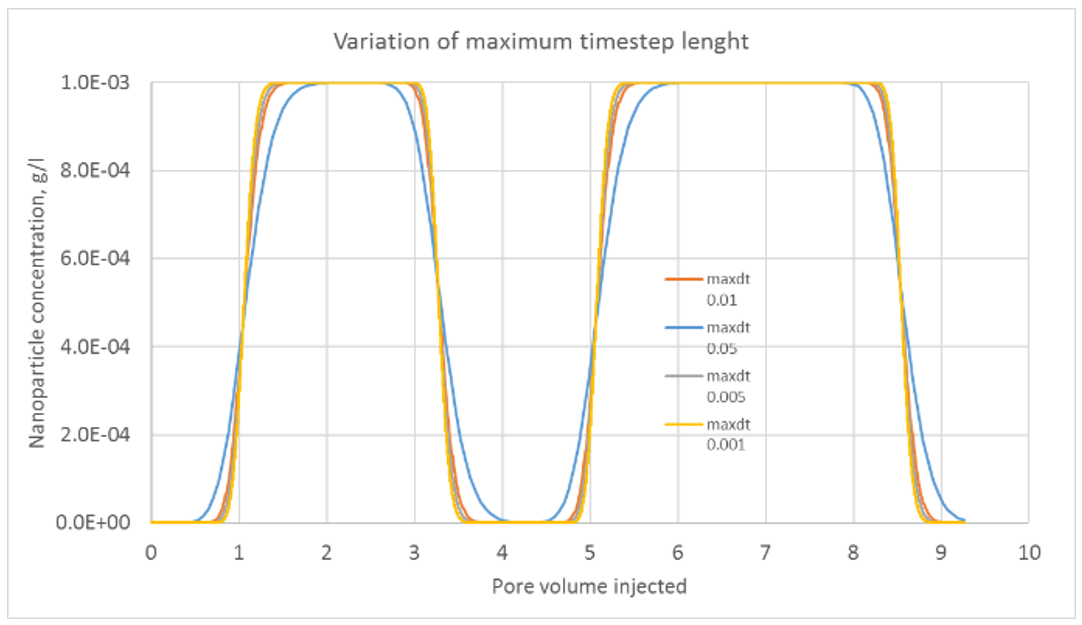
\includegraphics[width=\textwidth]{img/cht/simNPb.png}
    \caption{}
    \label{cht:simNPb}
    \end{subfigure}
    
    \caption{Concentration of nanoparticles as function of injected solution. Sensitivity simulations varying a) number of grid blocks in the model and b) maximum allowed time step length.}
    \label{cht:simNP}
\end{figure}

\begin{figure}[h] % figure 6.3
    \begin{subfigure}{\textwidth}
    \centering
    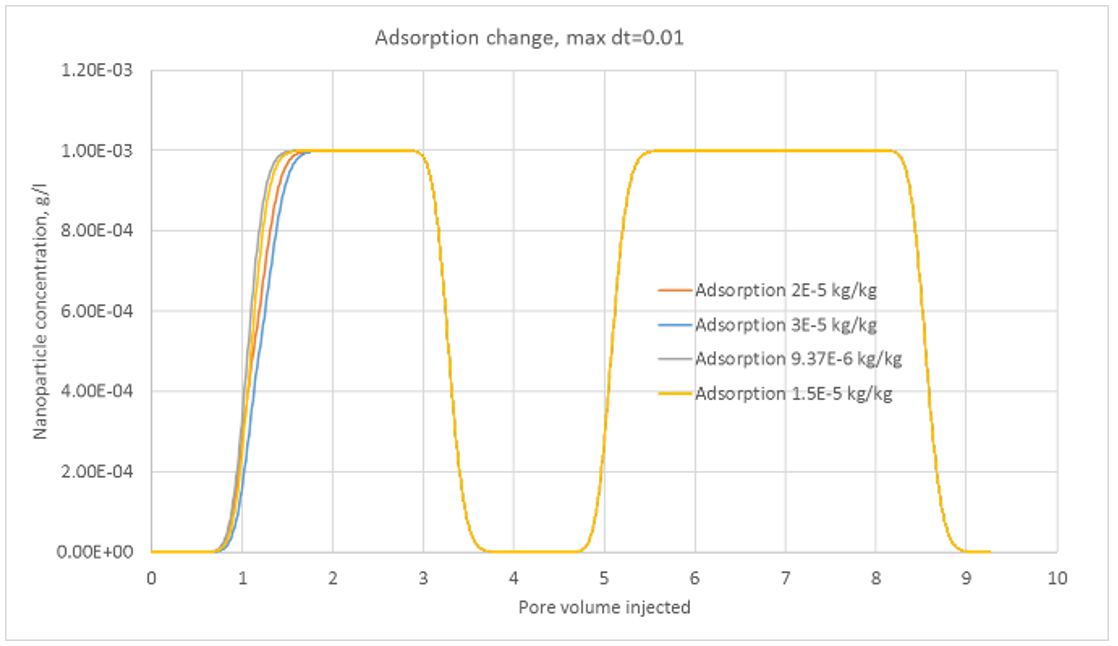
\includegraphics[width=\textwidth]{img/cht/simNPconcA.png}
    \caption{}
    \label{cht:simNPconcA}
    \end{subfigure}
    \\
    \begin{subfigure}{\textwidth}
    \centering
    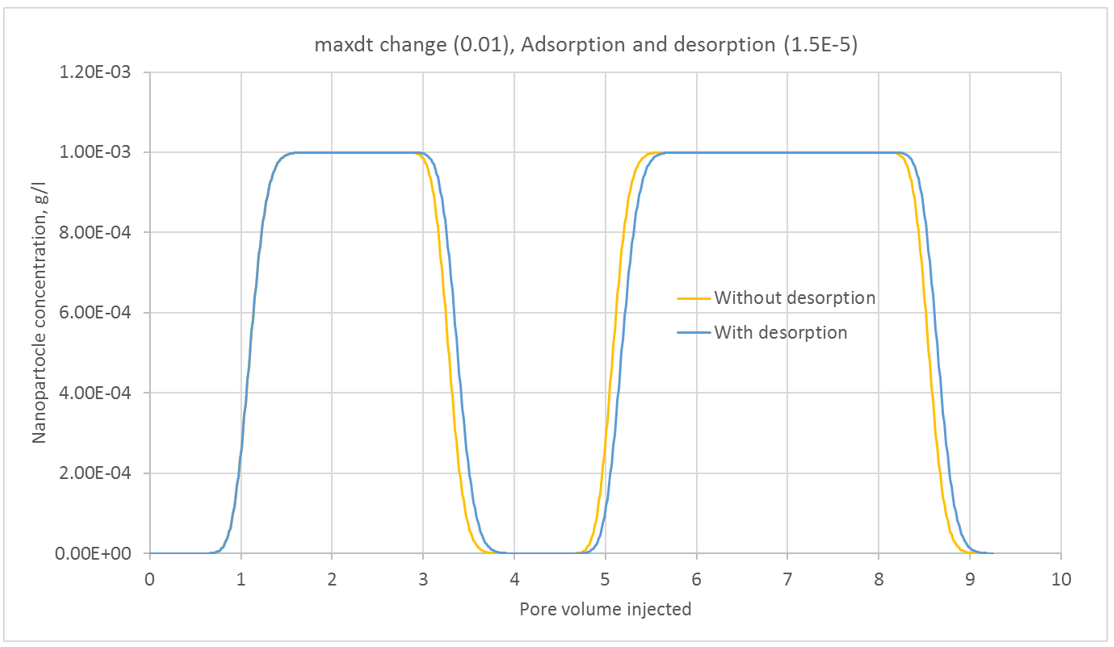
\includegraphics[width=\textwidth]{img/cht/simNPconcB.png}
    \caption{}
    \label{cht:simNPconcB}
    \end{subfigure}
    
    \caption{Concentration of nanoparticles as function of injected solution. Sensitivity simulations varying a) the adsorption isotherm for nanoparticles and b) with and without desorption of nanoparticles.}
    \label{cht:simNPconc}
\end{figure}

The next section describes results of simulating experiments performed on Bentheimer and Berea cores. The experiments targeted for simulation and history matching are listed in Table \ref{tab:crGels}.

\section{Simulation of laboratory experiments}

Experiment 1 to 3 injects solutions of nanoparticles and polymer in SSW into a Bentheimer sandstone core with permeability around 2.8 Darcy and porosity around 23\% (see Table \ref{tab:crGels}).

Experiment 1, nanoparticle injection into Bentheimer sandstone, injects two slugs with 1000 ppm nanoparticle (NP) concentration dissolved in synthetic sea water (SSW) each followed by SSW without NP. Inaccessible pore volume (IPV) for nanoparticles is assumed to be zero and the measured retention (0.010 mg/g rock) are taken into the adsorption isotherm. It is assumed that desorption of nanoparticles occurs for SSW flooding based on negative IPV for the SSW flooding (see Table \ref{tab:ipvexp1}). Figure \ref{cht:simExpNP} shows comparison of nanoparticle response from the simulation and the experiment for injection of nanoparticles into Bentheimer sandstone.

\begin{figure}[h]
    \centering
    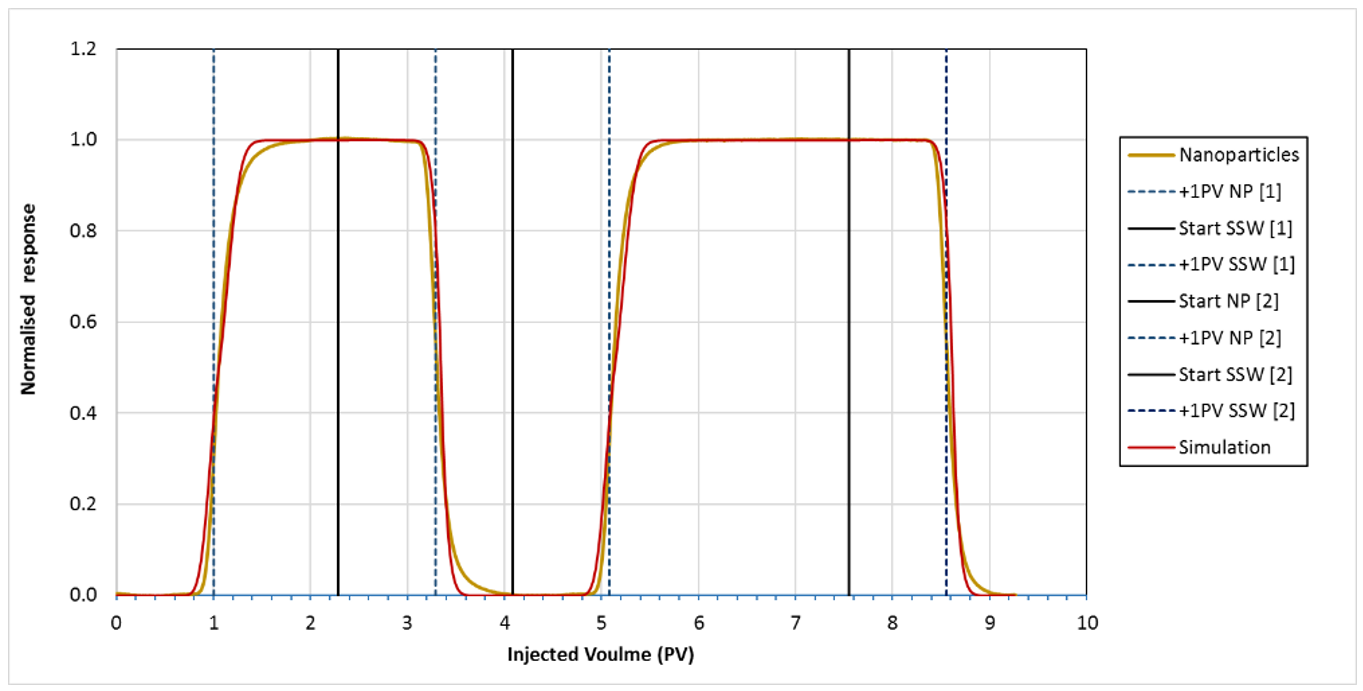
\includegraphics[width=\textwidth]{img/cht/simExpNP.png}
    \caption{Comparison of normalised nanoparticle concentration at the outlet of the core from experiment and from simulation of Experiment 1. The normalised nanoparticle response is plotted as function of injected PV.}
    \label{cht:simExpNP}
\end{figure}

Experiment 2, polymer injection into Bentheimer sandstone, injects two slugs of 1000 ppm polymer dissolved in SSW, each followed by SSW. For this case, an increase in viscosity as a function of polymer concentration and IPV for polymer is included in addition to adsorption of polymer on the rock surface. Adsorbed polymer also reduces absolute permeability in the rock. No desorption of polymer is assumed. Parameter input for the simulations are taken from Table \ref{tab:ipvexp2}, with IPV equal to 0.1 (average between 0.07 and 0.13) and adsorption coefficient at maximum polymer concentration equal to 0.02 mg/g rock (includes mechanical trapping). The reduction in absolute permeability for SSW with polymer is adjusted to match the differential pressure over the core. The viscosity of SSW as function of polymer concentration are taken from measurements giving a relative increase in viscosity by a factor of 4.31 at 1000 ppm polymer concentration. Figure \ref{cht:simExpNP2} shows comparison of normalised polymer response and differential pressure over the core/model from the simulation and experiment of polymer injection into Bentheimer sandstone.

\begin{figure}[h]
    \centering
    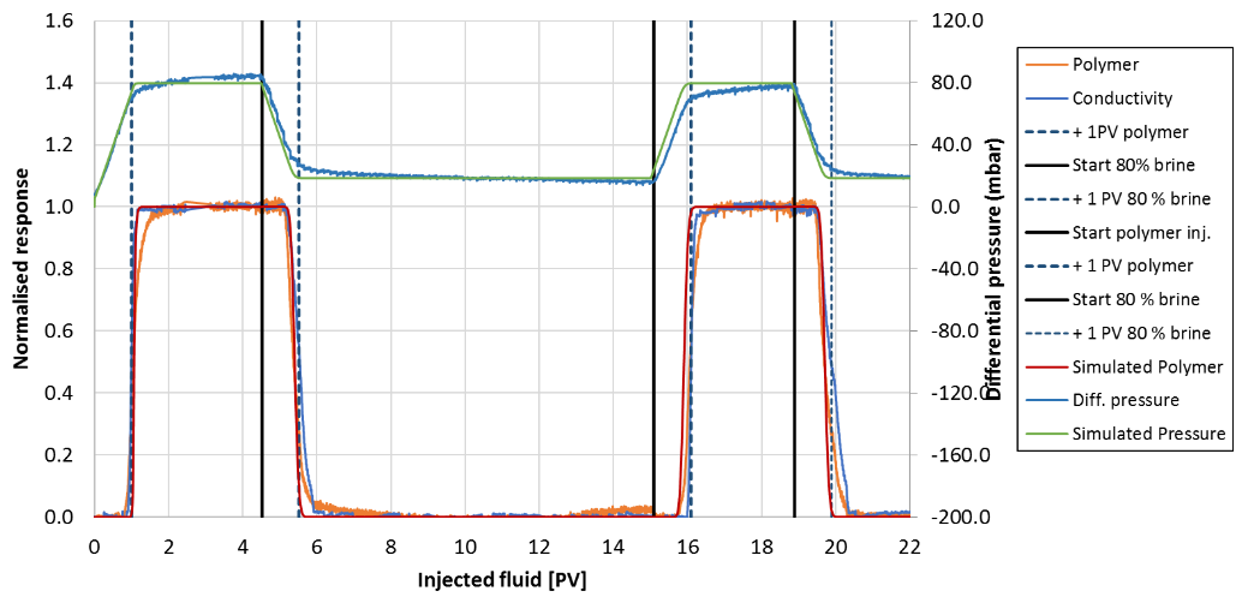
\includegraphics[width=\textwidth]{img/cht/simExpNP2.png}
    \caption{Comparison of normalised polymer concentration at the outlet of the core from experiment and from simulation of Experiment 2. Conductivity measurements from the experiment and differential pressure over the core is also plotted.}
    \label{cht:simExpNP2}
\end{figure}

Experiment 3 injects a solution with polymer and nanoparticles into Bentheimer sandstone. Two slugs with 2000 ppm nanoparticles and 500 ppm polymer were injected each followed by injection of SSW. Parameters for adsorption, IPV, permeability reduction and viscosity changes for nanoparticles and polymer are the same as for experiment 1 and 2, respectively. Figure \ref{cht:simExpNP3} shows simulation results compared to results from the experiment. Parameter input for the simulations are taken from Table \ref{tab:ipvexp3}.

\begin{figure}[h]
    \centering
    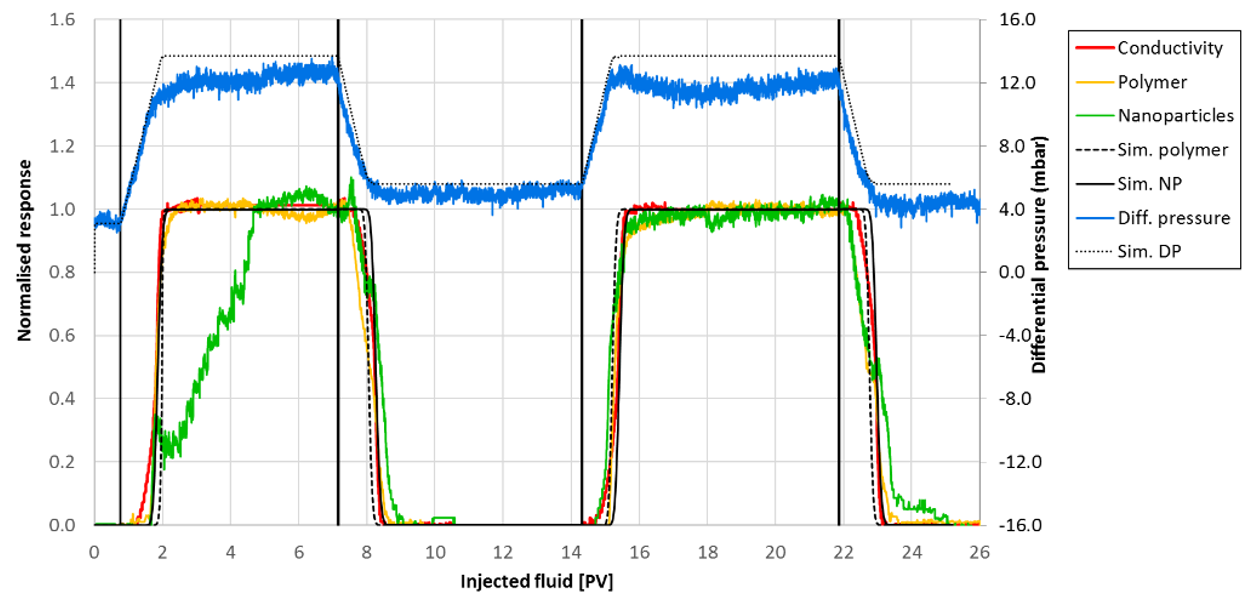
\includegraphics[width=\textwidth]{img/cht/simExpNP3.png}
    \caption{Comparison of experiment and simulation of co-injection of nanoparticles and polymer (Experiment 3). The nanoparticle response during the first injection slug in the experiment is assumed to be wrong. Conductivity measurements from the experiment and differential pressure over the core is also plotted.}
    \label{cht:simExpNP3}
\end{figure}

Experiments 4 – 6 follows the same schedule as experiment 1 – 3. Core material is now Berea sandstone with permeability around 0.3 Darcy and porosity around 19\% (see Table \ref{tab:ipvexp1}). From the experiments, it is apparent that the core is more heterogenous than the Bentheimer sandstone and that early breakthrough and tailing occurs (see for example Figure \ref{cht:CondBerNorm}). The effect of heterogeneity cannot be modelled correctly in the 1D simulator and results from the simulations will have a more "piston like" displacement. Figure \ref{cht:simExpNP4} and Figure \ref{cht:simExpNP5} compares nanoparticle and polymer response from measurement and simulation of experiments 4 and 5 respectively. 

\begin{figure}[h]
    \centering
    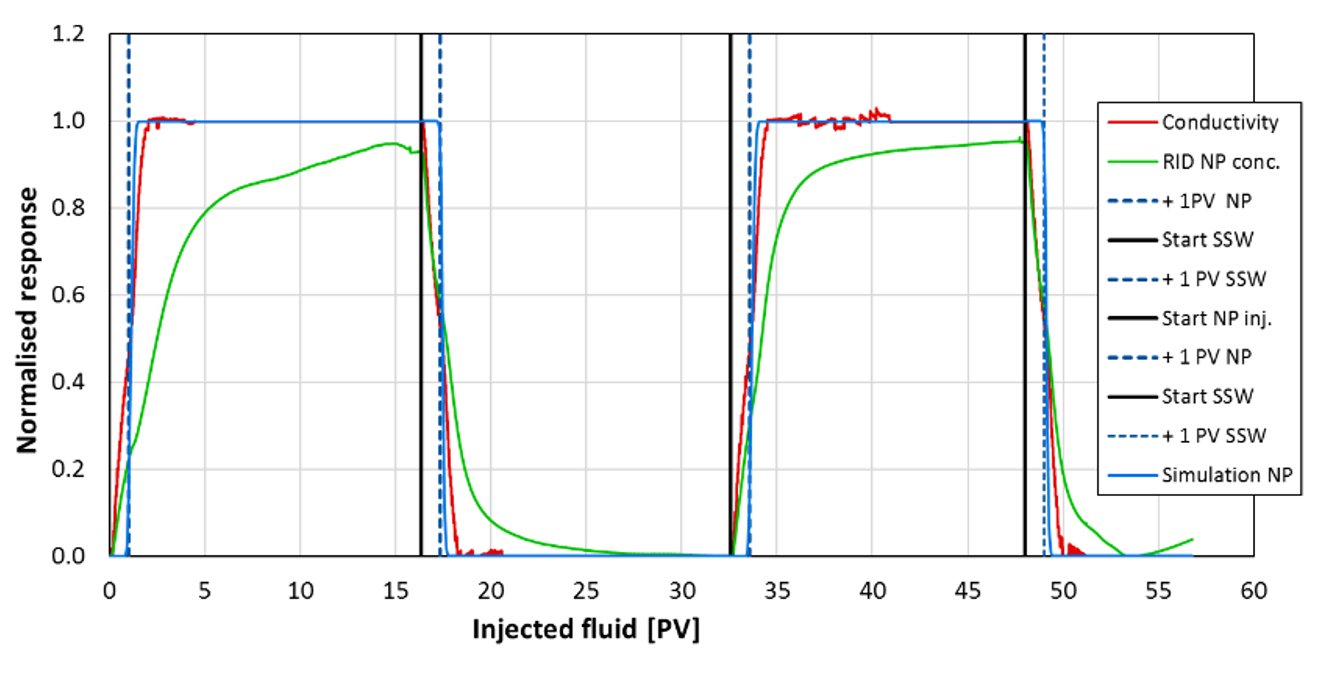
\includegraphics[width=\textwidth]{img/cht/simExpNP4.png}
    \caption{Comparison of normalised nanoparticle concentration from experiment 4 and from simulation of nanoparticle injection into Berea sandstone.}
    \label{cht:simExpNP4}
\end{figure}


\begin{figure}[h]
    \centering
    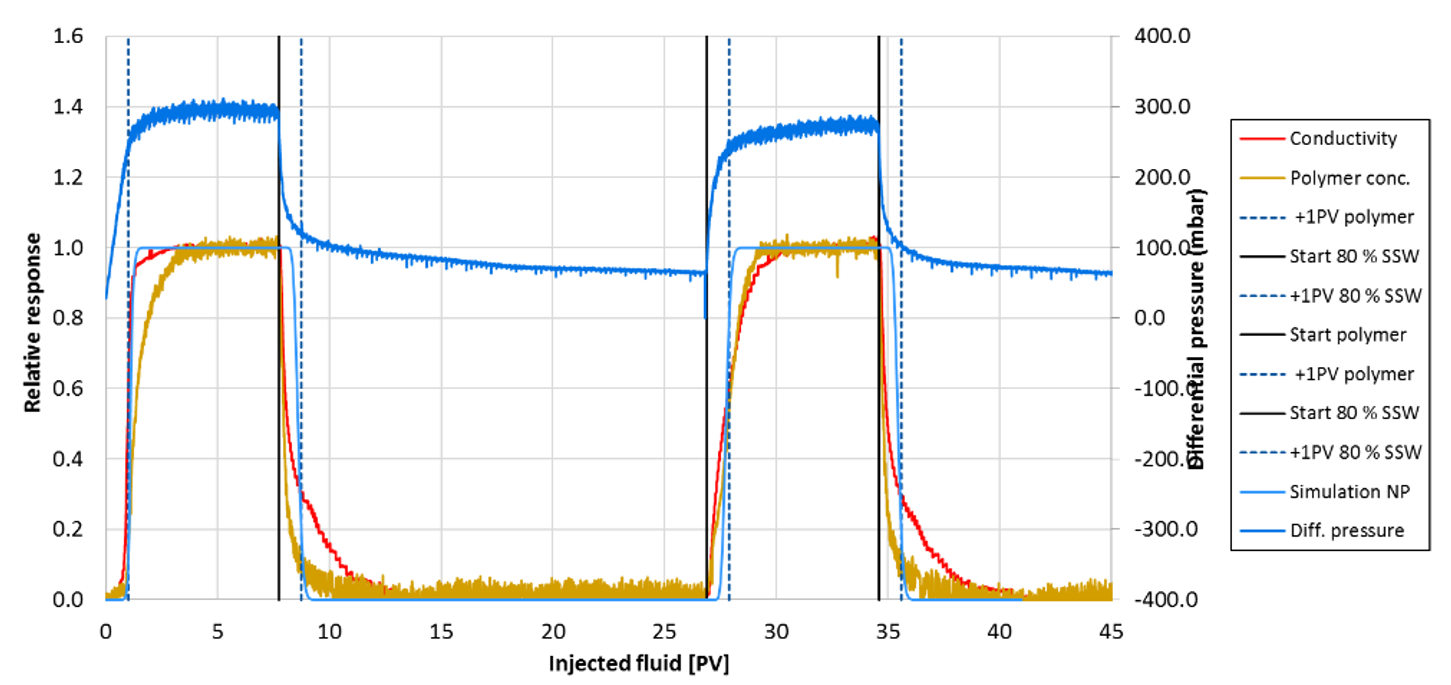
\includegraphics[width=\textwidth]{img/cht/simExpNP5.png}
    \caption{Comparison of normalised nanoparticle concentration from experiment 5 and from simulation of polymer injection into Berea sandstone.}
    \label{cht:simExpNP5}
\end{figure}

To compare the results from the developed 1D simulator with a commercial simulator and test the effect of heterogeneity, experiment 5 with injection of polymer into Berea sandstone has been simulated on 2D grids using ECLIPSE from Schlumberger. Three different models were constructed. One homogenous model with the same properties as used in the 1D model and two models with heterogenous permeability distribution. Permeability in the two heterogenous models varies between 100 and 400 mD, the first heterogenous model have constant permeability in layers (or tubes) while the second has a randomly distributed permeability (Figure \ref{cht:sim2dPerm}). 

\begin{figure}[h]
    \centering
    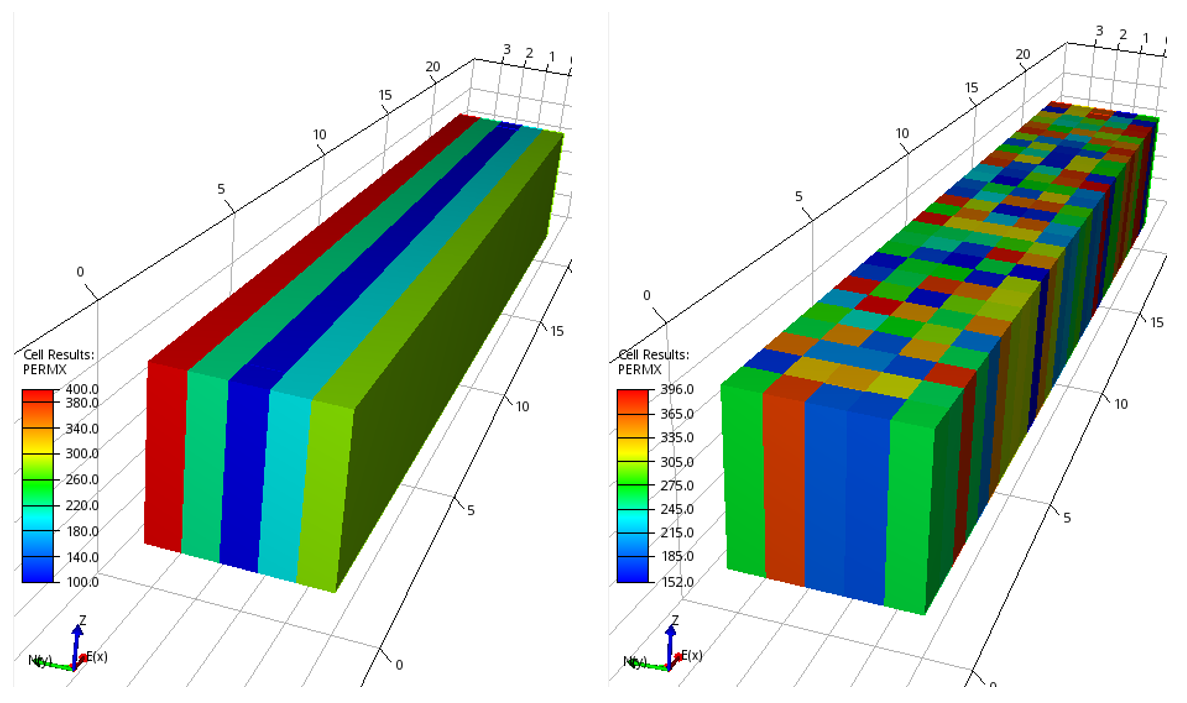
\includegraphics[width=\textwidth]{img/cht/sim2dPerm.png}
    \caption{Permeability distribution in the heterogenous 2D Eclipse models.}
    \label{cht:sim2dPerm}
\end{figure}

\enlargethispage{2cm} % add margin to bottom of this page
The ECLIPSE simulator has the functionality for modelling polymer injection in the aqueous phase and the same parameters as before for IPV, viscosity change as function of polymer concentration and adsorption of polymer, have been used. The results from the homogenous Eclipse simulation show a good match to the simulations from the developed 1D simulator (Figure \ref{cht:simEcl}).

\begin{figure}
    \centering
    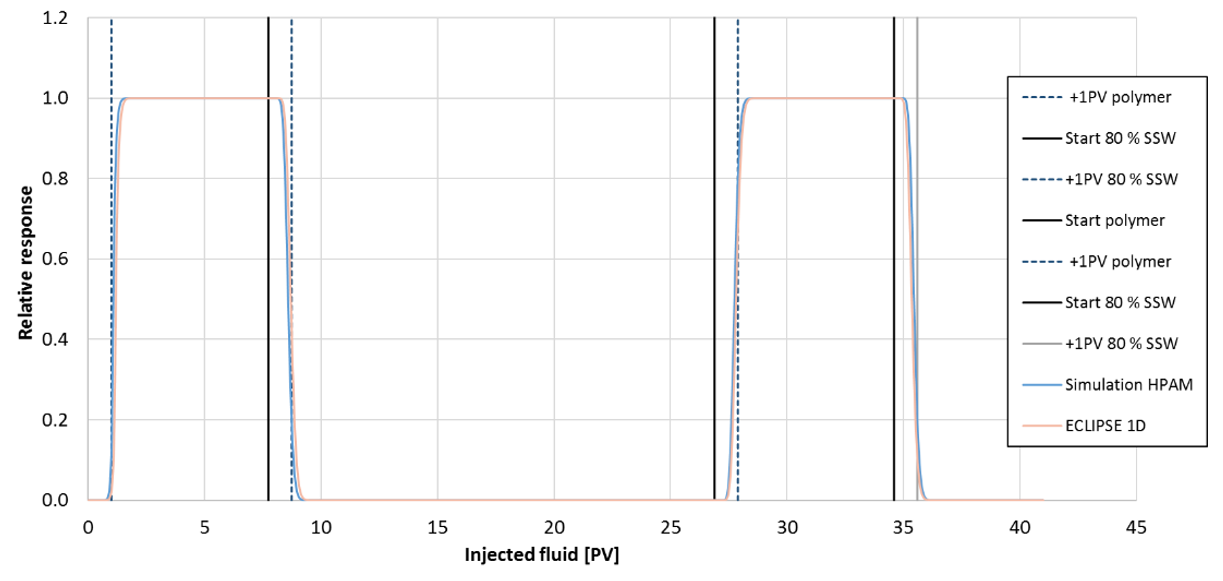
\includegraphics[width=\textwidth]{img/cht/simEcl.png}
    \caption{Comparison of polymer response between ECLIPSE and the developed simulator.}
    \label{cht:simEcl}
\end{figure}

\FloatBarrier

Results from adding simple heterogeneity to the ECLIPSE models are shown in Figure \ref{cht:simEclHet}. For the layered "pipe" model a tail in the polymer response is apparent at SSW break through after the first and second polymer flood. This is an effect of polymer flowing in layers with different permeabilities. There is also a smoothing of the polymer front at break through. Similar effects can be seen in the random permeability model but not to the same degree.    

\begin{figure}
    \centering
    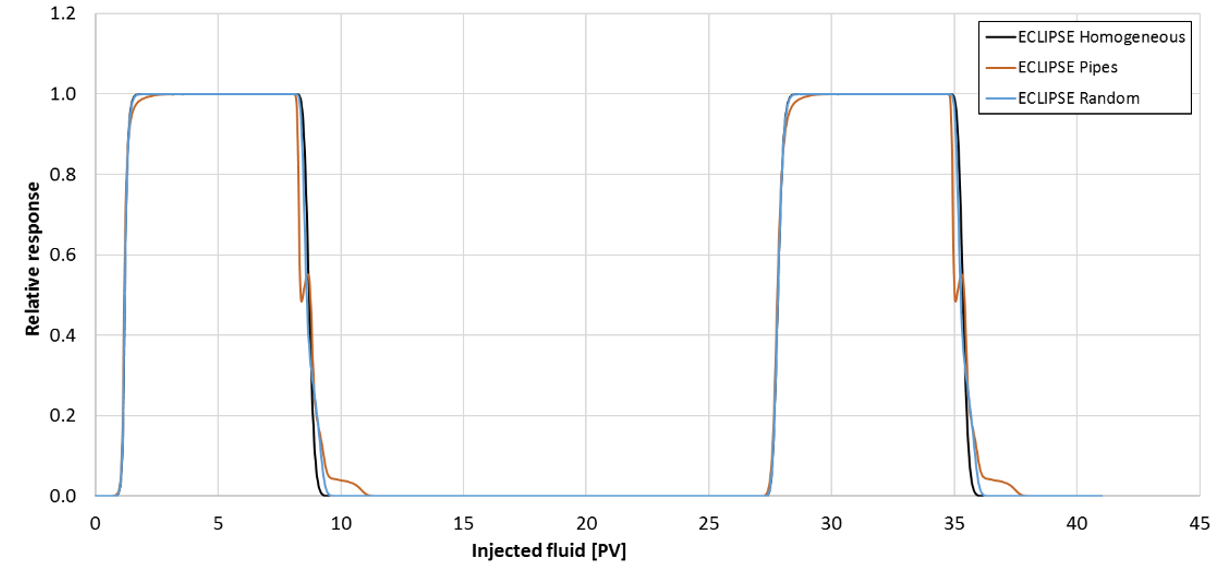
\includegraphics[width=\textwidth]{img/cht/simEclHet.png}
    \caption{Effect of heterogeneity in the ECLIPSE simulation models for polymer injection.}
    \label{cht:simEclHet}
\end{figure}

The effects of physical dispersion at the leading edge of the polymer slug and the fingering effects at the rear edge of the polymer slug is not implemented in the 1D simulator. Eclipse treats this with a Todd-Longstaff type mixing parameter,  $\omega$, for the effective water viscosity. The effective water viscosity is given as
\begin{equation}
    \mu_{p_\textit{eff}} = (\mu_m(C_p))^\omega \cdot \mu_p^{1-\omega}
\end{equation}
where the effective viscosity,  $\mu_{p_\textit{eff}}$, is a mix between the viscosity of a fully mixed polymer solution,  $\mu_m(C_p)$, and the viscosity of the solution at maximum polymer concentration,  $\mu_p$.  $\omega$ is the Todd-Longstaff mixing parameter which must be between 0 and 1.0. Figure \ref{cht:simEclMix} shows the polymer response in the homogeneous Eclipse model with mixing parameters 0.1, 0.5 and 1.0. Observe that using a mixing parameter less than one leads to dispersion in front and at the tail of the polymer slug.

No attempt was made to history match Experiment 6 with both polymer and nanoparticle injection into a Berea sandstone.

\begin{figure}
    \centering
    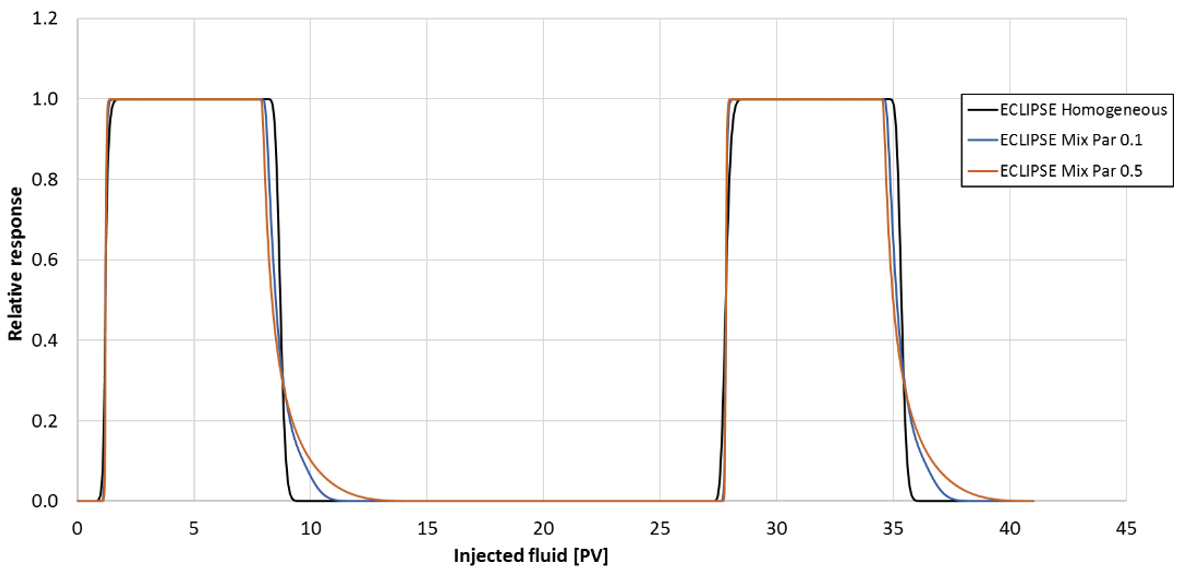
\includegraphics[width=\textwidth]{img/cht/simEclMix.png}
    \caption{Effect of using the mixing parameter for water viscosity in the ECLIPSE simulation models for polymer injection. }
    \label{cht:simEclMix}
\end{figure}

\section{Field scale modeling}
The full functionality of the simulator was tested by constructing a 100 m long simulation model with cross section 1 m$^2$. The simulation model has 1200 grid blocks, porosity and permeability was 0.24 and 2000 mD, respectively and the  IPV for polymer was set to 0.14. Otherwise, the parameters were as in experiment 3. Figure \ref{fig:largeScaleModel} shows an outline of the model.
\begin{figure}[h]
    \centering
    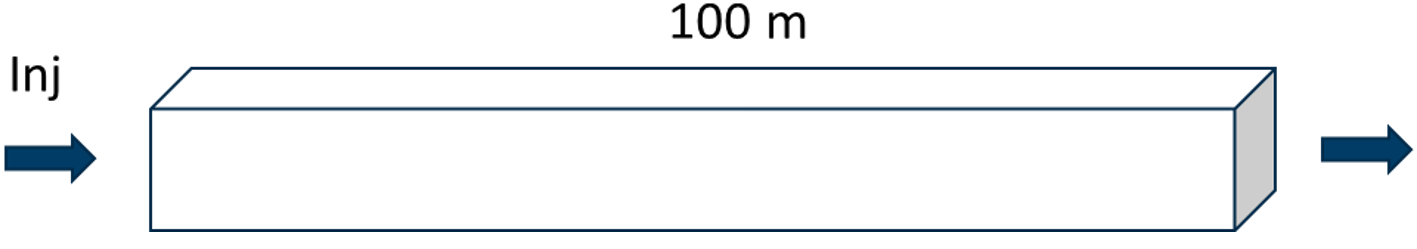
\includegraphics[width=\textwidth]{img/fig/largeScaleModel.png}
    \caption{Outline of the large-scale model. }
    \label{fig:largeScaleModel}
\end{figure}

Total pore volume (PV) of the model was 24 m$^3$ and an injection rate of 1 PV per 40 days were used (0.6 m$^3$/day). The schedule was set to inject a slug of 0.5 PV polymer and nanoparticle solution followed by 1.5 PV SSW. 

The applied \index{age function} age function for nanoparticles is shown in Figure \ref{cht:ageFunc} where nanoparticles start to crosslink the polymers at age 30 days. Full crosslinking effect for nanoparticles are reached after 33 days. Figure \ref{cht:hFunc} shows the two-variable function $h(C_p,C_n)$  reflecting the gel strength as function of polymer and nanoparticle concentrations.      

\begin{figure}[h] % figure 6.14
    \begin{subfigure}{\textwidth}
    \centering
    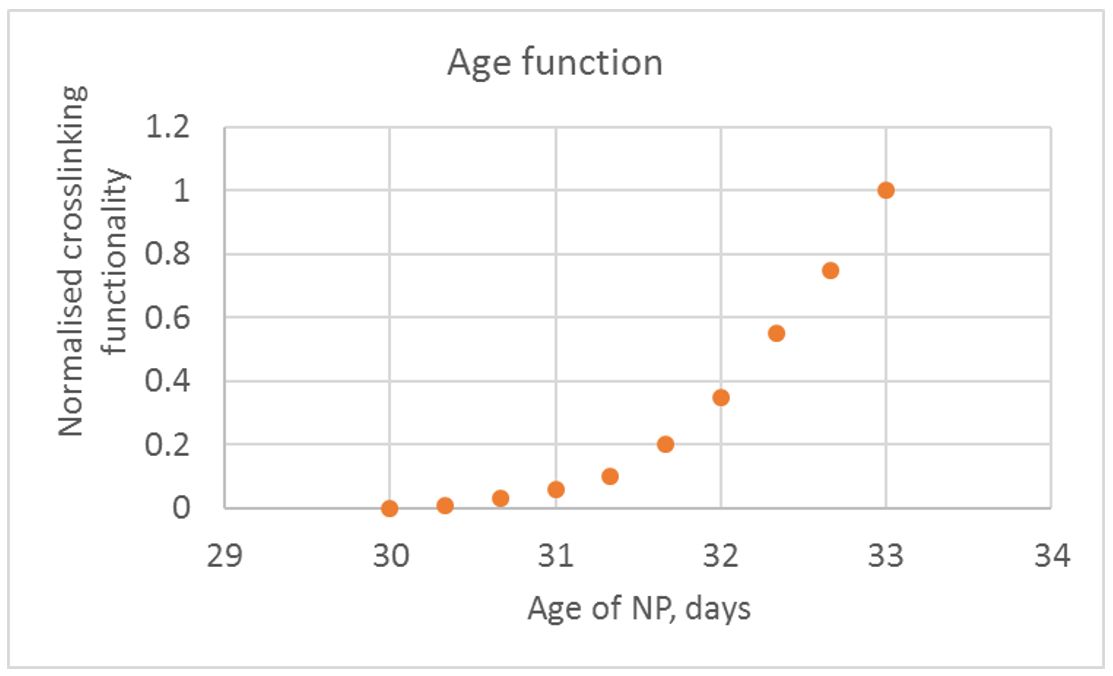
\includegraphics[width=\textwidth]{img/cht/ageFunc.png}
    \caption{}
    \label{cht:ageFunc}
    \end{subfigure}
    \\
    \begin{subfigure}{\textwidth}
    \centering
    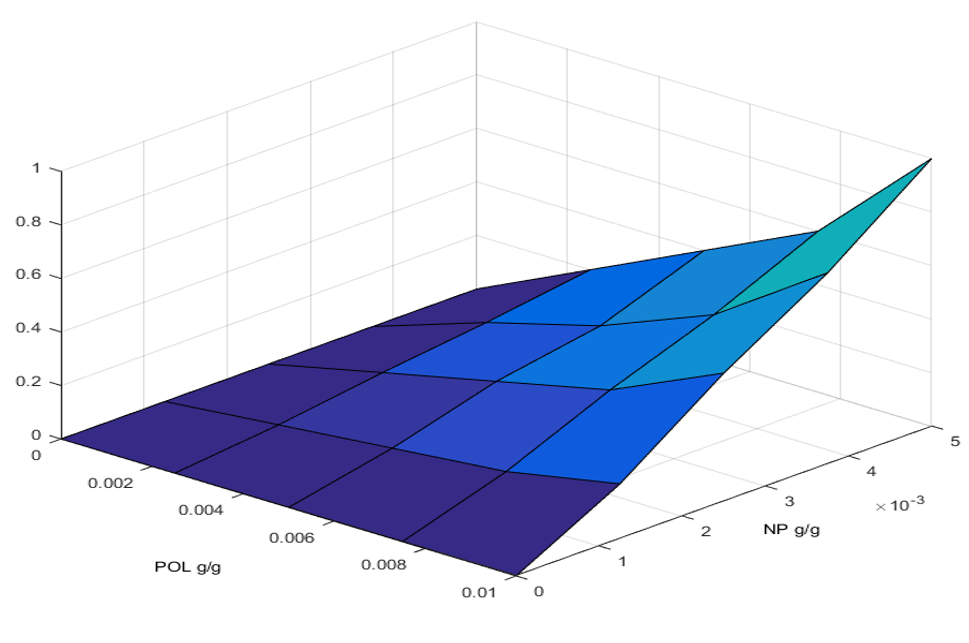
\includegraphics[width=\textwidth]{img/cht/hFunc.png}
    \caption{}
    \label{cht:hFunc}
    \end{subfigure}
    
    \caption{a) Age function for nanoparticles, $T_0$ is at 30 days and full crosslinking effect is reached at 33 days. b) $h$-function (see equation \ref{eq:ageEffect}), two parameter function of polymer and nanoparticle concentrations. }
    \label{cht:ageAndH}
\end{figure}

With the given nanoparticle age function the gelling should start at after 30 days, which corresponds to 75 m into the model. Maximum gel viscosity has been set to 50 cP to allow continued flooding of the 1D model after gel has formed. When gelling occurs in the model, a clear response on the differential pressure over the model should be noticed. Figure \ref{cht:pDiff} display differential pressure over the model and the relative concentrations of nanoparticle and polymer at the outlet of the model for injection of a) 0.5 PV polymer and nanoparticle solution and b) 0.25 PV polymer and nanoparticle solution followed by injection of SSW up to a total of 2 PV injected fluids. Both cases show an increase in differential pressure during solution injection due to increase in viscosity as function of polymer concentration. Reduction of effective permeability due to adsorption of polymer can be seen as a continued, but smaller increase in differential pressure until gelling occurs (at 0.75 PV injected or 75 m into the model) with a distinct increase in differential pressure. Observe that IPV and adsorption results in a splitting of the nanoparticle and polymer slugs and that for the case with slug size 0.25 PV only a smaller slug with high concentrations of both polymer and nanoparticles are produced at the outlet of the model. This is also reflected in a lower differential pressure over the model when gelling occurs.  

\begin{figure}[h] % figure 6.15
    \begin{subfigure}{.8\textwidth}
    \centering
    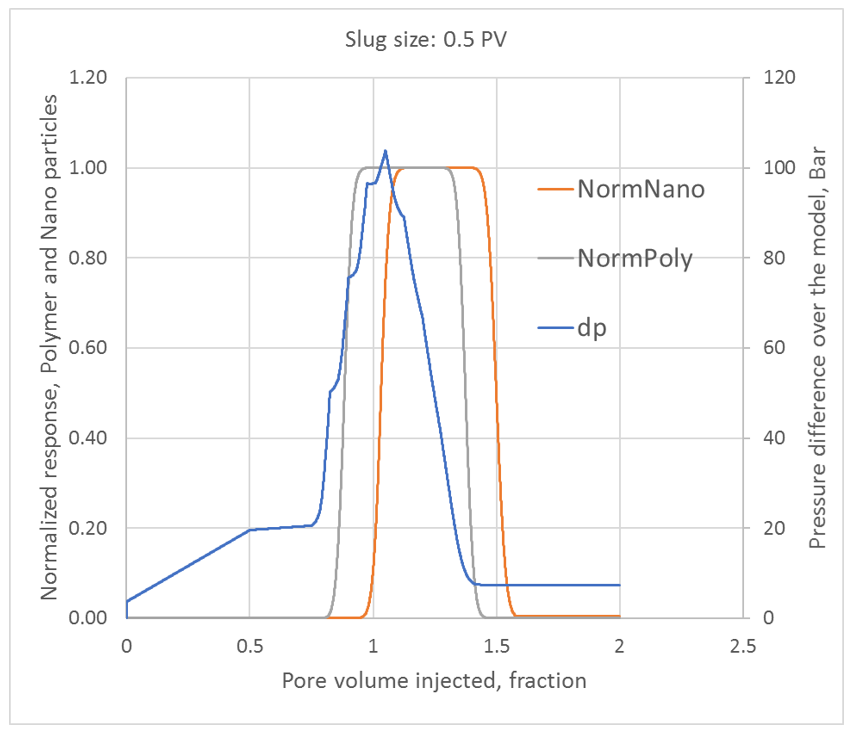
\includegraphics[width=\textwidth]{img/cht/pDiff1.png}
    \caption{}
    \label{cht:pDiff1}
    \end{subfigure}
    \\
    \begin{subfigure}{.8\textwidth}
    \centering
    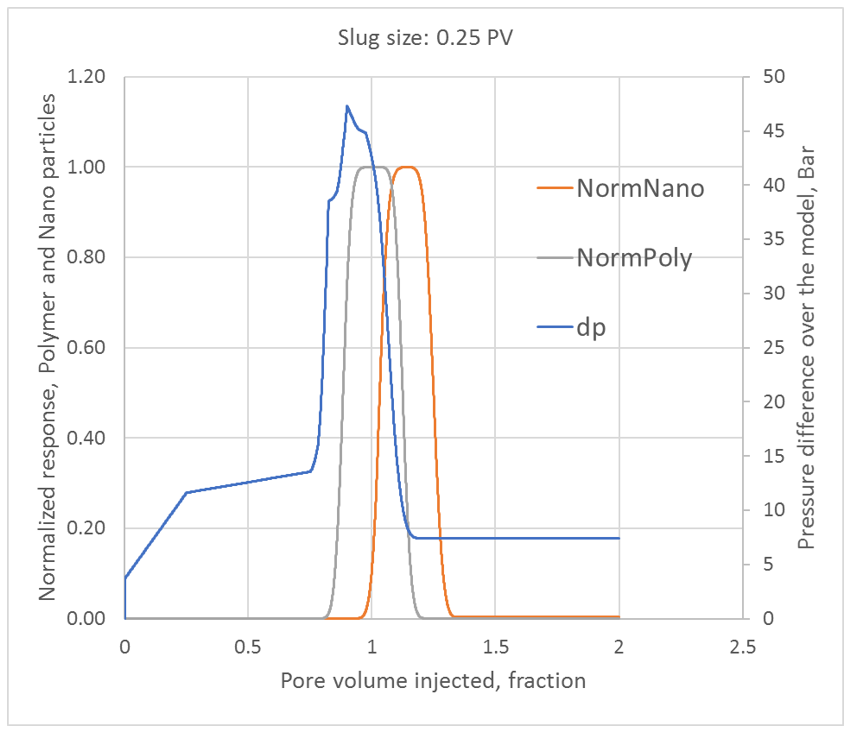
\includegraphics[width=\textwidth]{img/cht/pDiff2.png}
    \caption{}
    \label{cht:pDiff2}
    \end{subfigure}
    
    \caption{Differential pressure response for the large scale gelling simulation with a) injection of 0.5 PV polymer and nanoparticle slug and b) injection of 0.25 PV polymer and nanoparticle slug, both followed by SSW injection. }
    \label{cht:pDiff}
\end{figure}